\chapter{Méthodes de pénalité et Lagrangien augmenté}
\label{chap:penalty-augmented-lagrangian}

\section{La méthode de pénalité quadratique}

\subsection{Motivation}

\textbf{Idée :} Remplacer les contraintes par des \textbf{pénalités non négatives} que l'on ajoute à la fonction objectif.

Considérons le problème général :
\begin{equation}
    \min_{x \in \mathbb{R}^n} f(x) \quad \text{sujet à} \quad
    \begin{cases}
        c_i(x) = 0, & i \in \mathcal{E} \\
        c_i(x) \ge 0, & i \in \mathcal{I}
    \end{cases}
\end{equation}

Définissons la \textbf{fonction de pénalité quadratique} comme :
\begin{equation}
    Q(x; \mu) = f(x) + \frac{\mu}{2} \sum_{i \in \mathcal{E}} c_i(x)^2 + \frac{\mu}{2} \sum_{i \in \mathcal{I}} \left[ c_i(x)^- \right]^2
\end{equation}
où $x^- = \max(-x, 0)$ et $\mu > 0$ est le \textbf{paramètre de pénalité}.

L'idée est de remplacer le problème contraint par un problème \textbf{non contraint} :
\begin{equation}
    \min_{x \in \mathbb{R}^n} Q(x; \mu)
\end{equation}
La fonction objectif de ce sous-problème contient :
\begin{itemize}
    \item la fonction objectif originale $f(x)$;
    \item un terme additionnel pour chaque contrainte, qui est positif si la contrainte est violée, et nul sinon.
\end{itemize}

\begin{remarque}
    À cause des contraintes d'inégalité, le nouveau problème est \textbf{moins lisse} à cause de la fonction max.
\end{remarque}

\begin{figure}[H]
\centering
\begin{tikzpicture}[scale=1.5]
    \draw[->] (-2.5,0) -- (1.5,0) node[right] {$x$};
    \draw[->] (0,-0.5) -- (0,2.5);
    
    \draw[thick, red] (-2, 2) -- (0, 0) -- (1, 0);
    \node[red, above left] at (-1.8, 2.0) {$x \mapsto x^-$};
    
    \draw[thick, teal, domain=-1.5:0] plot (\x, {\x*\x});
    \draw[thick, teal] (0, 0) -- (1, 0);
    \node[teal, below left] at (-1.4, 2.0) {$x \mapsto (x^-)^2$};
    
    % Dashed lines for x=-1
    \draw[dashed, gray] (-1, 0) node[below] {$-1$} -- (-1, 1);
    \draw[dashed, gray] (-1, 1) -- (0, 1) node[right] {$1$};
    
    % Origin
    \node[below right] at (0,0) {$0$};
    
\end{tikzpicture}
\caption{Comparaison des fonctions de pénalité pour une inégalité $x \ge 0$. En rouge, la pénalité exacte $x^-$ (non différentiable en 0). En vert, la pénalité quadratique $(x^-)^2$ (différentiable, $C^1$).}
\label{fig:penalty-functions-comparison}
\end{figure}

\begin{figureexplanation}
La pénalité linéaire $x^-$ présente une cassure à l'origine (non différentiable), tandis que $(x^-)^2$ est lisse et tangente à l'axe. Cette différentiabilité permet d'appliquer les méthodes de gradient.
\end{figureexplanation}

\paragraph{Exemple :}
Soit $\min_{x \in \mathbb{R}^2} x_1 + x_2$ sujet à $x_1^2 + x_2^2 - 2 = 0$.
La fonction de pénalité quadratique est :
\begin{equation}
    Q(x; \mu) = x_1 + x_2 + \frac{\mu}{2} (x_1^2 + x_2^2 - 2)^2
\end{equation}
Le gradient s'annule lorsque (avec $x_1 = x_2$ par symétrie) :
\begin{equation}
    1 + 4\mu x_1 (x_1^2 - 1) = 0
\end{equation}
Il existe un minimum local qui tend vers $(-1, -1)$ lorsque $\mu \to \infty$.

\begin{figure}[H]
\centering
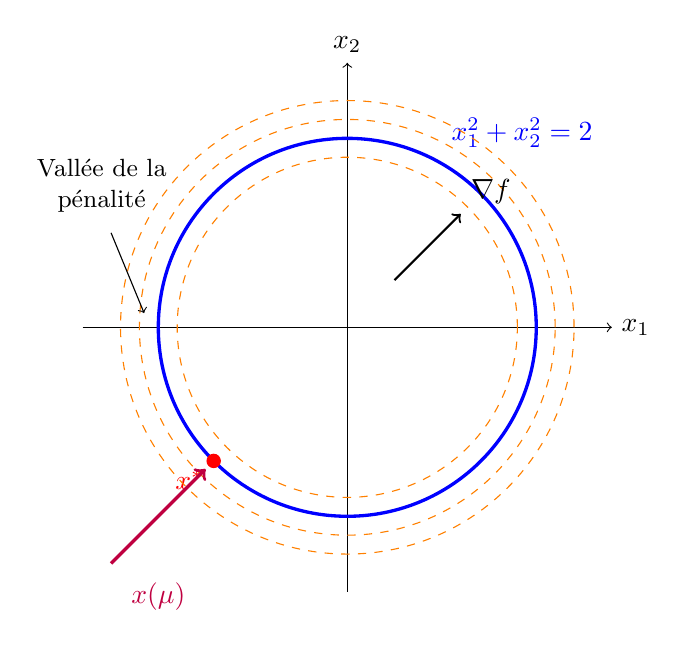
\begin{tikzpicture}[scale=1.2]
    \draw[->] (-2.8,0) -- (2.8,0) node[right] {$x_1$};
    \draw[->] (0,-2.8) -- (0,2.8) node[above] {$x_2$};
    
    \draw[very thick, blue] (0,0) circle (2);
    \node[blue, above right] at (1.0, 1.8) {$x_1^2+x_2^2=2$};
    \filldraw[red] (-1.414, -1.414) circle (2pt) node[below left] {$x^*$};
    
    % Penalty Contours
    \draw[orange, thin, dashed] (0,0) circle (2.2);
    \draw[orange, thin, dashed] (0,0) circle (1.8);
    \draw[orange, thin, dashed] (0,0) circle (2.4);
    
    \draw[->, black, thick] (0.5, 0.5) -- (1.2, 1.2) node[above right] {$\nabla f$};
    
    \draw[->, purple, very thick] (-2.5, -2.5) -- (-1.5, -1.5);
    \node[purple, below] at (-2.0, -2.6) {$x(\mu)$};
    
    \node[align=center, font=\small] at (-2.6, 1.5) {Vallée de la\\pénalité};
    \draw[->] (-2.5, 1.0) -- (-2.15, 0.15);
    
\end{tikzpicture}
\caption{Méthode de pénalité : Lorsque $\mu$ augmente, la fonction $Q(x;\mu)$ forme une "vallée" abrupte le long de la contrainte $c(x)=0$. La suite de minimiseurs $x(\mu)$ (flèche violette) descend au fond de cette vallée tout en se rapprochant de la contrainte, pour finir en $x^*$.}
\label{fig:penalty-valley}
\end{figure}

\begin{figureexplanation}
\textbf{La "vallée" de pénalité :}
Imaginez que la contrainte (le cercle bleu) est le fond d'un canyon.
\begin{itemize}
    \item Loin du cercle, le terme de pénalité $\frac{\mu}{2} c(x)^2$ est immense : les murs du canyon sont très hauts.
    \item Pour minimiser $Q$, il faut descendre au fond du canyon ($c(x) \approx 0$).
    \item Une fois au fond, on cherche à minimiser la fonction originale $f(x)$ en se déplaçant \emph{le long} de la contrainte.
    \item Problème numérique : Le fond est un peu "plat" dans la direction de la contrainte, mais les murs sont très raides. Cela crée une matrice Hessienne mal conditionnée ("longue et étroite").
\end{itemize}
\end{figureexplanation}

\begin{algorithm}[H]
    \caption{Méthode de pénalité quadratique}
    \SetAlgoLined
    Données : $\mu_0 > 0$, une suite positive $(\tau_k)_k$ avec $\tau_k \to 0$, et un point de départ $x_0^s$\;
    \For{$k=0, 1, \ldots$}{
        Trouver un minimiseur approximatif $x_k$ de $Q(\cdot;\mu_k)$, en partant de $x_k^s$ et en terminant lorsque $\|\nabla_x Q(x;\mu_k)\|\leq \tau_k$\;
        \If{critère d'arrêt final satisfait}{
            \Stop avec la solution approximative $x_k$\;
        }
        Choisir un nouveau paramètre de pénalité $\mu_{k+1} > \mu_k$\;
        Choisir un nouveau point de départ $x_{k+1}^s$\;
    }
\end{algorithm}

\subsection{Convergence de la méthode (avec contraintes d'égalité)}

\begin{theoreme}[Convergence Globale]
    Supposons que chaque $x_k$ est le minimiseur exact de $Q(\cdot; \mu_k)$ et que $\mu_k \uparrow \infty$.
    Alors, tout point limite $x^*$ de la suite $(x_k)_k$ est une solution globale du problème.
\end{theoreme}

\begin{proof}
    Soit $\bar{x}$ une solution globale du problème contraint.
    Alors $\bar{x}$ est admissible, c'est-à-dire $c_i(\bar{x}) = 0$ pour tout $i \in \mathcal{E}$.
    Par définition de $x_k$ comme minimiseur de $Q(\cdot; \mu_k)$, on a :
    \[
        Q(x_k; \mu_k) \le Q(\bar{x}; \mu_k).
    \]
    En développant l'expression de la fonction de pénalité :
    \[
        f(x_k) + \frac{\mu_k}{2} \sum_{i \in \mathcal{E}} c_i(x_k)^2 \le f(\bar{x}) + \frac{\mu_k}{2} \sum_{i \in \mathcal{E}} c_i(\bar{x})^2.
    \]
    Puisque $\bar{x}$ est admissible, le terme de pénalité pour $\bar{x}$ est nul :
    \[
        f(x_k) + \frac{\mu_k}{2} \sum_{i \in \mathcal{E}} c_i(x_k)^2 \le f(\bar{x}).
    \]
    Réarrangons cette inégalité pour isoler le terme de violation des contraintes :
    \[
        \sum_{i \in \mathcal{E}} c_i(x_k)^2 \le \frac{2}{\mu_k} [f(\bar{x}) - f(x_k)].
    \]
    Supposons que $x^*$ est un point limite de la suite $(x_k)_k$. Il existe une sous-suite $\mathcal{K}$ telle que :
    \[
        \lim_{k \in \mathcal{K}} x_k = x^*.
    \]
    Prenons la limite dans l'inégalité précédente pour $k \in \mathcal{K}$ tendant vers l'infini. Comme $\mu_k \to \infty$, le terme de droite tend vers 0 (en supposant $f(x_k)$ borné ou convergent vers $f(x^*)$) :
    \[
        \sum_{i \in \mathcal{E}} c_i(x^*)^2 = \lim_{k \in \mathcal{K}} \sum_{i \in \mathcal{E}} c_i(x_k)^2 \le 0.
    \]
    Comme une somme de carrés est toujours positive ou nulle, on en déduit que $\sum c_i(x^*)^2 = 0$, et donc :
    \[
        c_i(x^*) = 0, \quad \forall i \in \mathcal{E}.
    \]
    Ainsi, $x^*$ est un point admissible.
    
    De plus, reprenons l'inégalité $f(x_k) + \text{pénalité} \le f(\bar{x})$. Comme le terme de pénalité est positif, on a simplement :
    \[
        f(x_k) \le f(\bar{x}).
    \]
    En passant à la limite sur la sous-suite $\mathcal{K}$ :
    \[
        f(x^*) \le f(\bar{x}).
    \]
    Puisque $x^*$ est admissible et que sa valeur objective est inférieure ou égale à celle de la solution globale $\bar{x}$, $x^*$ est lui-même une solution globale.
\end{proof}

\begin{remarque}
    En pratique, trouver le minimiseur exact n'est pas réaliste à chaque étape.
\end{remarque}

\begin{theoreme}[Convergence KKT]
    Supposons que les tolérances et les pénalités satisfont $\tau_k \downarrow 0$ et $\mu_k \uparrow \infty$.
    Alors, si un point limite $x^*$ de la suite $(x_k)_k$ est \textbf{inadmissible} (infeasible), alors $x^*$ est un point stationnaire de la fonction $x \mapsto \|c(x)\|^2 = \sum_{i \in \mathcal{E}} [c_i(x)]^2$.
    
    D'autre part, si $x^*$ est \textbf{admissible} (feasible) et si les gradients des contraintes $\nabla c_i(x^*)$ sont linéairement indépendants (LICQ), alors $x^*$ est un point KKT pour le problème.
\end{theoreme}

\begin{remarque}[Multiplicateurs de Lagrange]
    Pour de tels points, pour tout sous-ensemble d'indices $\mathcal{K}$ tel que $x^* = \lim_{k \in \mathcal{K}} x_k$, on a :
    \[
        \lim_{k \in \mathcal{K}} (-\mu_k c_i(x_k)) = \lambda_i^*, \quad \text{pour tout } i \in \mathcal{E},
    \]
    où $\lambda^*$ sont les multiplicateurs de Lagrange associés à $x^*$ pour le problème original.
    \begin{proof}
        Voir Nocedal et Wright.
    \end{proof}
\end{remarque}

\begin{remarque}[Mal-conditionnement de la Hessienne]
    La Hessienne de la fonction de pénalité est donnée par :
    \[
        \nabla_{xx}^2 Q(x; \mu_k) = \nabla^2 f(x) + \sum_{i \in \mathcal{E}} \mu_k c_i(x) \nabla^2 c_i(x) + \mu_k A(x)^\top A(x),
    \]
    où $A(x)^\top = [\nabla c_i(x)]_{i \in \mathcal{E}}$.
    
    Lorsque $x$ est proche du minimiseur de $Q(\cdot; \mu_k)$, les conditions du théorème sont satisfaites et on a l'approximation :
    \[
        \nabla_{xx}^2 Q(x; \mu_k) \approx \nabla_{xx}^2 \mathcal{L}(x, \lambda^*) + \mu_k A(x)^\top A(x).
    \]
    La matrice $\nabla_{xx}^2 \mathcal{L}(x, \lambda^*)$ est indépendante de $\mu_k$.
    Le terme $\mu_k A(x)^\top A(x)$ est de rang $|\mathcal{E}|$ (car $A(x)$ a $|\mathcal{E}|$ lignes qui sont les gradients supposés indépendants).
    
    Ainsi, la Hessienne possède $|\mathcal{E}|$ valeurs propres d'ordre $\mu_k$ (provenant de $A^\top A$) et $n - |\mathcal{E}|$ valeurs propres d'ordre 1 (provenant du Lagrangien).
    Cette matrice est singulière lorsque $|\mathcal{E}| < n$ pour le terme dominant.
    
    Puisque $\mu_k \to \infty$, le conditionnement de la matrice explose : $\nabla_{xx}^2 Q(\cdot; \mu_k)$ devient mal conditionnée (ill-conditioned). Cela rend la minimisation par des méthodes de Newton ou quasi-Newton difficile.
\end{remarque}

\paragraph{Conséquence sur le calcul du pas de Newton :}
    On cherche à résoudre $\nabla_{xx}^2 Q(x; \mu_k) p_N = -\nabla_x Q(x; \mu_k)$.
    Pour éviter les erreurs numériques dues au mauvais conditionnement, on introduit une variable auxiliaire $\zeta = \mu_k A(x) p_N$.
    Le système peut alors être réécrit sous la forme :
    \[
    \begin{pmatrix}
        \nabla^2 f(x) + \sum_{i \in \mathcal{E}} \mu_k c_i(x) \nabla^2 c_i(x) & A(x)^\top \\
        A(x) & -\frac{1}{\mu_k} I
    \end{pmatrix}
    \begin{pmatrix}
        p_N \\
        \zeta
    \end{pmatrix}
    =
    \begin{pmatrix}
        -\nabla_x Q(x; \mu_k) \\
        0
    \end{pmatrix}
    \]
    Cette formulation évite de former explicitement la matrice mal conditionnée $\mu_k A^\top A$.

\section{Fonctions de pénalité non lisses ($l^1$)}

\subsection{Définition et propriétés}

Une alternative populaire est la fonction de pénalité $l^1$, définie par :
\[
    \phi_1(x; \mu) = f(x) + \mu \sum_{i \in \mathcal{E}} |c_i(x)| + \mu \sum_{i \in \mathcal{I}} [c_i(x)]^-,
\]
où $[y]^- = \max(-y, 0)$.

Contrairement à la pénalité quadratique, cette fonction n'est pas différentiable aux points où $c_i(x) = 0$. Cependant, elle possède une propriété très importante : c'est une \textbf{fonction de pénalité exacte}.

\begin{theoreme}[Pénalité Exacte]
    Supposons que $x^*$ soit une solution locale stricte du problème contraint :
    \[
        \min f(x) \quad \text{s.c. } \quad c_i(x) = 0, \; i \in \mathcal{E}, \quad c_i(x) \ge 0, \; i \in \mathcal{I},
    \]
    et que les conditions KKT du premier ordre soient satisfaites pour des multiplicateurs $\lambda^*$.
    
    Alors, $x^*$ est un minimum local de $\phi_1(\cdot; \mu)$ pour tout $\mu > \mu^*$, où
    \[
        \mu^* = \|\lambda^*\|_\infty = \max_i |\lambda_i^*|.
    \]
    Si les conditions suffisantes du second ordre sont également satisfaites, alors $x^*$ est un minimum local \textbf{strict}.
\end{theoreme}

\begin{figure}[H]
    \centering
    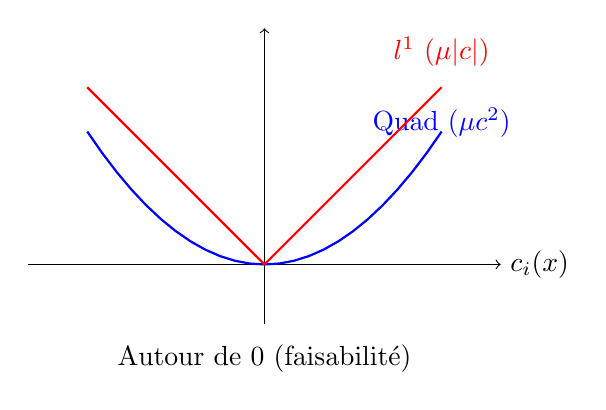
\begin{tikzpicture}[scale=1.5]
        \draw[->] (-2,0) -- (2,0) node[right] {$c_i(x)$};
        \draw[->] (0,-0.5) -- (0,2);
        
        \draw[blue, thick, domain=-1.5:1.5] plot (\x, {0.5*\x*\x});
        \node[blue] at (1.5, 1.2) {Quad ($\mu c^2$)};
        
        % L1
        \draw[red, thick] (-1.5, 1.5) -- (0,0) -- (1.5, 1.5);
        \node[red] at (1.5, 1.8) {$l^1$ ($\mu |c|$)};
        
        \node[align=center] at (0, -0.8) {Autour de $0$ (faisabilité)};
    \end{tikzpicture}
    \caption{Comparaison : La pénalité quadratique (bleue) est lisse mais a une pente nulle à l'origine, nécessitant $\mu \to \infty$ pour forcer $c(x) \to 0$. La pénalité $l^1$ (rouge) a une pente non nulle ("kink") à l'origine, permettant une solution exacte pour $\mu$ fini.}
\end{figure}

\subsection{Caractérisation du comportement}

Nous souhaitons étudier les points stationnaires de $\phi_1$, qui n'est pas différentiable.
Pour cela, nous utilisons les dérivées directionnelles.

\begin{definition}[Dérivée directionnelle]
    La dérivée directionnelle de $f: \mathbb{R}^n \to \mathbb{R}$ dans la direction $p \in \mathbb{R}^n$ est donnée par :
    \[
        D(f(x), p) = \lim_{\epsilon \to 0} \frac{f(x + \epsilon p) - f(x)}{\epsilon}.
    \]
\end{definition}

\begin{definition}[Stationnarité]
    Un point $\hat{x} \in \mathbb{R}^n$ est un point stationnaire pour la fonction de pénalité $\phi_1(\cdot; \mu)$ si :
    \[
        D(\phi_1(\hat{x}; \mu), p) \ge 0, \quad \text{pour tout } p \in \mathbb{R}^n.
    \]
\end{definition}

Nous définissons également une mesure de l'inadmissibilité (infeasibility measure) :
\[
    h(x) = \sum_{i \in \mathcal{E}} |c_i(x)| + \sum_{i \in \mathcal{I}} [c_i(x)]^-.
\]
Un point $\hat{x}$ est un "point stationnaire pour la mesure d'inadmissibilité" si $D(h(\hat{x}); p) \ge 0$ pour tout $p \in \mathbb{R}^n$.
Si de plus $x$ est inadmissible pour le problème original, on dit que c'est un \textbf{point stationnaire inadmissible}.

\begin{theoreme}
    Supposons que $\hat{x}$ est un point stationnaire pour la fonction de pénalité $\phi_1(\cdot; \mu)$ pour tout $\mu > \mu^*$.
    Alors :
    \begin{itemize}
        \item Si $\hat{x}$ est admissible pour le problème, alors il satisfait les conditions KKT.
        \item Sinon, c'est un point stationnaire inadmissible.
    \end{itemize}
\end{theoreme}

\begin{exemple}
    Considérons le problème :
    \[
        \min_{x \in \mathbb{R}^2} x_1 + x_2 \quad \text{s.c.} \quad x_1^2 + x_2^2 - 2 = 0.
    \]
    La fonction de pénalité $l^1$ est :
    \[
        \phi_1(x; \mu) = x_1 + x_2 + \mu |x_1^2 + x_2^2 - 2|.
    \]
    On peut montrer que le minimiseur de $\phi_1(\cdot; \mu)$ est la solution $(-1, -1)$ pour tout $\mu > \mu^* = 0.5$.
\end{exemple}

\section{Approche pratique : Modèle $l^1$ modifié}

Comme $\phi_1(\cdot; \mu)$ n'est pas lisse, on ne peut pas appliquer directement la méthode de Newton.
Une approche pratique (Framework 20) consiste à former un modèle modifié en :
\begin{itemize}
    \item Linéarisant les contraintes $c_i$.
    \item Remplaçant $f$ par une approximation quadratique.
\end{itemize}
On cherche alors à minimiser par rapport à $p$ la fonction :
\[
    q(p; \mu) = f(x) + \nabla f(x)^\top p + \frac{1}{2} p^\top W p + \mu \sum_{i \in \mathcal{E}} |c_i(x) + \nabla c_i(x)^\top p| + \mu \sum_{i \in \mathcal{I}} [c_i(x) + \nabla c_i(x)^\top p]^-,
\]
où $W$ est une approximation de la Hessienne du Lagrangien.
Ce modèle $q(p; \mu)$ n'est pas lisse. Cependant, si $W$ est définie positive, on peut reformuler ce sous-problème en un problème quadratique lisse (QP) en introduisant des variables artificielles $r, s, t$ :
\[
    \min_{p, r, s, t} \nabla f(x)^\top p + \frac{1}{2} p^\top W p + \mu \sum_{i \in \mathcal{E}} (r_i + s_i) + \mu \sum_{i \in \mathcal{I}} t_i
\]
sous les contraintes :
\[
    \begin{cases}
        \nabla c_i(x)^\top p + c_i(x) = r_i - s_i, & i \in \mathcal{E} \\
        \nabla c_i(x)^\top p + c_i(x) \ge -t_i, & i \in \mathcal{I} \\
        r, s, t \ge 0
    \end{cases}
\]
Ce problème peut être résolu efficacement par des solveurs QP standards.

\section{Méthodes du Lagrangien Augmenté}

\subsection{Définition et Motivation}

Nous avons vu que pour la pénalité quadratique, la suite $\{x_k\}$ converge vers une solution, mais il faut que $\mu_k \to \infty$. Cela entraîne un mauvais conditionnement de la Hessienne.
De plus, on a la relation asymptotique :
\[
    \lim_{k \to \infty} -\mu_k c_i(x_k) = \lambda_i^*.
\]
L'idée des méthodes de Lagrangien Augmenté est d'utiliser une estimation explicite des multiplicateurs de Lagrange $\lambda$ pour éviter de devoir faire tendre $\mu$ vers l'infini trop rapidement.

On définit le \textbf{Lagrangien Augmenté} $\mathcal{L}_A$ par :
\[
    \mathcal{L}_A(x, \lambda; \mu) = f(x) - \sum_{i \in \mathcal{E}} \lambda_i c_i(x) + \frac{\mu}{2} \sum_{i \in \mathcal{E}} c_i(x)^2.
\]
Cette fonction combine le Lagrangien et la pénalité quadratique.

\subsection{Algorithme (Méthode des Multiplicateurs)}

L'algorithme proposé est le suivant :
\begin{enumerate}
    \item À l'étape $k$, on fixe une estimation des multiplicateurs $\lambda^k$ et une pénalité $\mu_k > 0$.
    \item On cherche un minimiseur $x_k$ de $\mathcal{L}_A(\cdot, \lambda^k; \mu_k)$. La condition d'optimalité est :
    \[
        \nabla_x \mathcal{L}_A(x_k, \lambda^k; \mu_k) = \nabla f(x_k) - \sum_{i \in \mathcal{E}} (\lambda_i^k - \mu_k c_i(x_k)) \nabla c_i(x_k) \approx 0.
    \]
    \item En comparant avec la condition KKT $\nabla f(x^*) - \sum \lambda_i^* \nabla c_i(x^*) = 0$, cela suggère la règle de mise à jour suivante pour les multiplicateurs :
    \[
        \lambda_i^{k+1} = \lambda_i^k - \mu_k c_i(x_k).
    \]
\end{enumerate}

\paragraph{Comparaison du comportement :}
\begin{itemize}
    \item \textbf{Avant (Pénalité quadratique seule) :} On avait $-\mu_k c_i(x_k) \approx \lambda_i^*$, ce qui impliquait $c_i(x_k) \approx -\frac{\lambda_i^*}{\mu_k}$. Pour avoir $c_i$ petit, il fallait $\mu_k$ très grand.
    \item \textbf{Avec Lagrangien Augmenté :} La condition devient $\lambda_i^k - \mu_k c_i(x_k) \approx \lambda_i^*$.
    Ainsi :
    \[
        c_i(x_k) \approx \frac{\lambda_i^k - \lambda_i^*}{\mu_k}.
    \]
    Si $\lambda^k$ converge vers $\lambda^*$, le numérateur tend vers 0. On peut donc obtenir une petite violation des contraintes $c_i(x_k)$ même sans que $\mu_k$ tende vers l'infini.
\end{itemize}



\section{Méthode du Lagrangien augmenté}

\subsection{Propriétés du cas avec contraintes d'égalité}

\begin{algorithm}[H]
    \caption{Augmented Lagrangian method for equality constraints}
    \SetAlgoLined
    Given $\mu_0>0$, tolerance $\tau_0>0$, starting points $x_0^s$ and $\lambda^0$\;
    \For{$k=0, 1, \ldots$}{
        Find an approximate minimizer $x_k$ of $\mathcal{L}_A(\cdot, \lambda^k;\mu_k)$, starting at $x_k^s$, and terminating when $\|\nabla_x \mathcal{L}_A(x_k, \lambda^k; \mu_k)\| \leq \tau_k$\;
        \If{a convergence test for the equality-constrained problem is satisfied}{
            \Stop with approximate solution $x_k$\;
        }
        Update Lagrange multipliers using
        \[
            \lambda_i^{k+1} = \lambda_i^k - \mu_k c_i(x_k), \text{ for all } i\in\mathcal{E};
        \]
        Choose new penalty parameter $\mu_{k+1} \geq \mu_k$\;
        Set starting point for the next iteration to $x_{k+1}^s = x_k$\;
        Select tolerance $\tau_{k+1}$\;
    }
\end{algorithm}

\subsection{Méthodes pratiques du Lagrangien augmenté}

\subsubsection{Formulation avec contraintes de bornes}

\begin{algorithm}[H]
    \caption{Bound-constrained Lagrangian method}
    \SetAlgoLined
    Choose an initial point $x_0$ and initial multipliers $\lambda^0$\;
    Choose convergence tolerances $\eta_*$ and $\omega_*$\;
    Set $\mu_0=10$, $\omega_0=\frac{1}{\mu_0}$, and $\eta_0=\frac{1}{\mu_0^{0.1}}$\;
    \For{$k=0,1, \ldots$}{
        Find an approximate solution $x_k$ of the problem
        \[
            \min_x \mathcal{L}_A(x,\lambda^k;\mu_k) \text{ subject to } l\leq x\leq u
        \]
        such that
        \[
            \left\| x_k-P\left(x_k - \nabla_x \mathcal{L}_A(x_k, \lambda^k ; \mu_k), l, u\right) \right\| \leq \omega_k;
        \]
        \If{$\|c(x_k)\|\leq \eta_k$}{
            \Comment{test for convergence}
            \If{$\|c(x_k)\|\leq \eta_*$ \And $\left\| x_k-P\left(x_k - \nabla_x \mathcal{L}_A(x_k, \lambda^k ; \mu_k), l, u\right) \right\| \leq \omega_*$}{
                \Stop with approximate solution $x_k$\;
            }
            \Comment{update multipliers, tighten tolerances}
            $\lambda^{k+1}\leftarrow \lambda^k - \mu_k c(x_k)$\;
            $\mu_{k+1}\leftarrow \mu_k$\;
            $\eta_{k+1}\leftarrow \frac{\eta_k}{\mu_{k+1}^{0.9}}$\;
            $\omega_{k+1} \leftarrow \frac{\omega_k}{\mu_{k+1}}$\;
        }
        \Else{
            \Comment{increase penalty parameters, tighten tolerances}
            $\lambda^{k+1}\leftarrow \lambda^k$\;
            $\mu_{k+1}\leftarrow 100 \mu_k$\;
            $\eta_{k+1}\leftarrow \frac{1}{\mu_{k+1}^{0.1}}$\;
            $\omega_{k+1} \leftarrow \frac{1}{\mu_{k+1}}$\;
        }
    }
\end{algorithm}



%%%%%%%%%%%%%%%%%%%%%%%%%%%%%%%%%%%%%%%%%%%%%%%%%%%%%%%%%%%%
\section{Exercices d'entraînement (Nocedal \& Wright)}
\label{sec:12.exercises}

Exercices relatifs au chapitre 17 du livre (Penalty and Augmented Lagrangian Methods).

\bigskip
\begin{exercice}[Convergence de la méthode de pénalité quadratique]
Vérifier que si $x^*$ est solution du problème contraint, alors c'est un point stationnaire de la fonction de pénalité quadratique $Q(x; \mu)$ lorsque $\mu \to \infty$. 
(Voir Théorème 17.1 et exercice 17.1 du livre).
\end{exercice}

\begin{correction}
$\nabla Q(x; \mu) = \nabla f(x) + \mu \sum c_i(x) \nabla c_i(x)$.
Pour que $\nabla Q \to 0$, il faut que $\nabla f$ soit balancé par le terme de pénalité.
En limite, $x_k \to x^*$.
Si $x^*$ est réalisable, $c_i(x^*) = 0$.
La relation limite donne $\nabla f(x^*) + \sum \lambda_i^* \nabla c_i(x^*) = 0$ (KKT), où $\lambda_i^* \approx -\mu c_i(x_k)$.
\end{correction}
\bigskip

\bigskip
\begin{exercice}[Comparaison Lagrangien Augmenté vs Pénalité]
Étudier l'Exemple 17.4 (page 536 du livre Nocedal/Wright) qui compare le conditionnement des deux méthodes pour le problème :
$$ \min x_1 + x_2 \quad \text{s.c. } x_1^2 + x_2^2 - 2 = 0 $$
Montrer que le Lagrangien Augmenté converge mieux et avec un meilleur conditionnement que la pénalité simple.
\end{exercice}

\begin{correction}
Le cercle $x_1^2 + x_2^2 = 2$ est la contrainte. Solution $x^*=(-1,-1)$.
Pénalité simple : les contours deviennent très allongés ("vallée") autour de la contrainte, rendant la minimisation difficile (mauvais conditionnement de la hessienne).
Lagrangien Augmenté : Le terme linéaire $-\lambda^\top c(x)$ "décale" le fond de la vallée pour qu'il coïncide avec la contrainte sans avoir besoin d'un $\mu$ immense.
Cela permet de trouver la solution précise avec un $\mu$ modéré, donc un meilleur conditionnement.
\end{correction}
\bigskip

\bigskip
\begin{exercice}[Calcul explicite - Méthode de Pénalité]
Considérer le problème scalaire :
$$ \min_{x \in \mathbb{R}} \frac{1}{2}x^2 \quad \text{s.c. } x = 1 $$
\begin{enumerate}
    \item Écrire la fonction de pénalité quadratique $Q(x; \mu)$.
    \item Trouver le minimiseur $x_\mu$ de $Q(x; \mu)$ pour $\mu > 0$ donné.
    \item Vérifier que $x_\mu \to x^*$ (la solution exacte) quand $\mu \to \infty$.
    \item Estimer le multiplicateur de Lagrange $\lambda^*$ à partir de $x_\mu$ et vérifier sa convergence.
\end{enumerate}
\end{exercice}

\begin{correction}
\textbf{1. Fonction de pénalité :}
$Q(x; \mu) = \frac{1}{2}x^2 + \frac{\mu}{2}(x-1)^2$.

\textbf{2. Minimiseur $x_\mu$ :}
$Q'(x) = x + \mu(x-1) = 0$.
$x(1+\mu) = \mu \implies x_\mu = \frac{\mu}{1+\mu}$.

\textbf{3. Convergence Primate :}
$\lim_{\mu \to \infty} x_\mu = \lim \frac{\mu}{\mu} = 1$.
La solution exacte du problème est évidemment $x^*=1$. Convergence vérifiée.

\textbf{4. Multiplicateur Dual :}
KKT exact : $L = \frac{1}{2}x^2 - \lambda(x-1)$. $\nabla L = x - \lambda = 0 \implies \lambda^* = x^* = 1$.
Estimation pénalité (Formule $\lambda \approx -\mu c(x)$ pour $L = f - \lambda c$) :
$\lambda_\mu = -\mu (x_\mu - 1) = -\mu (\frac{\mu}{1+\mu} - 1) = -\mu (\frac{\mu - (1+\mu)}{1+\mu}) = -\mu (\frac{-1}{1+\mu}) = \frac{\mu}{1+\mu}$.
Quand $\mu \to \infty$, $\lambda_\mu \to 1$.
Convergence vérifiée vers $\lambda^* = 1$.
\end{correction}
\bigskip

\bigskip
\begin{checkpoint}
\begin{itemize}
    \item \textbf{Pénalité Quadratique :} Pourquoi $\mu \to \infty$ pose-t-il problème ? (Conditionnement de la Hessienne).
    \item \textbf{Pénalité $l^1$ :} Quel est son avantage principal par rapport à la quadratique ? (Pénalité exacte pour $\mu$ fini).
    \item \textbf{Inconvénient $l^1$ :} Quel est le prix à payer pour l'exactitude ? (Fonction non différentiable à la solution).
    \item \textbf{Lagrangien Augmenté :} Quel est l'avantage principal par rapport à la pénalité simple ? (Convergence des multiplicateurs sans $\mu$ infini).
    \item \textbf{Mise à jour :} Comment met-on à jour $\lambda$ dans la méthode du Lagrangien Augmenté ? ($\lambda \leftarrow \lambda - \mu c(x)$).
\end{itemize}
\end{checkpoint}

